\chapter{Loss Functions in Deep Learning are non-convex}\label{chp:Loss Functions in Deep Learning are non-convex}
% Authors: tn1050@nyu.edu, vy404@nyu.edu, sk7685@nyu.edu.
% Lecture date: 2.4.19

Things like regression for single layer are convex and the function you are optimizing is quadratic in x. However
loss functions of pretty much every multi-layer network are non-convex and have multiple local minima.
Luckily, it is shown that these local minima are all more or less equivalent. 
When we train a neural net with different initial conditions then the solutions we get at the end are very different to each other. 
However performances of all the solutions will be more or less the same. 

\section{Example: Identity Function}
% Authors: tn1050@nyu.edu, vy404@nyu.edu, sk7685@nyu.edu.
% Lecture date: 2.4.19
The figure the loss surface of a two layer neural net with one input, one hidden unit and one output and the network tries to approximate the identity function. 
The input and the output are both 0.5. The cost function is squared error 
\begin{equation}
    L = (0.5 - \tanh (W_1 \tanh (W_0 * 0.5)))^2
\end{equation}
% L = (0.5 - tanh(W_1 tanh (W_0*0.5)))^2 
The objective function looks as follows in the space of $W_1$, $W_2$. 
We get a saddle point at (0,0) where curvature is positive in two directions and negative in two.\\

\begin{figure}[ht]
\centering
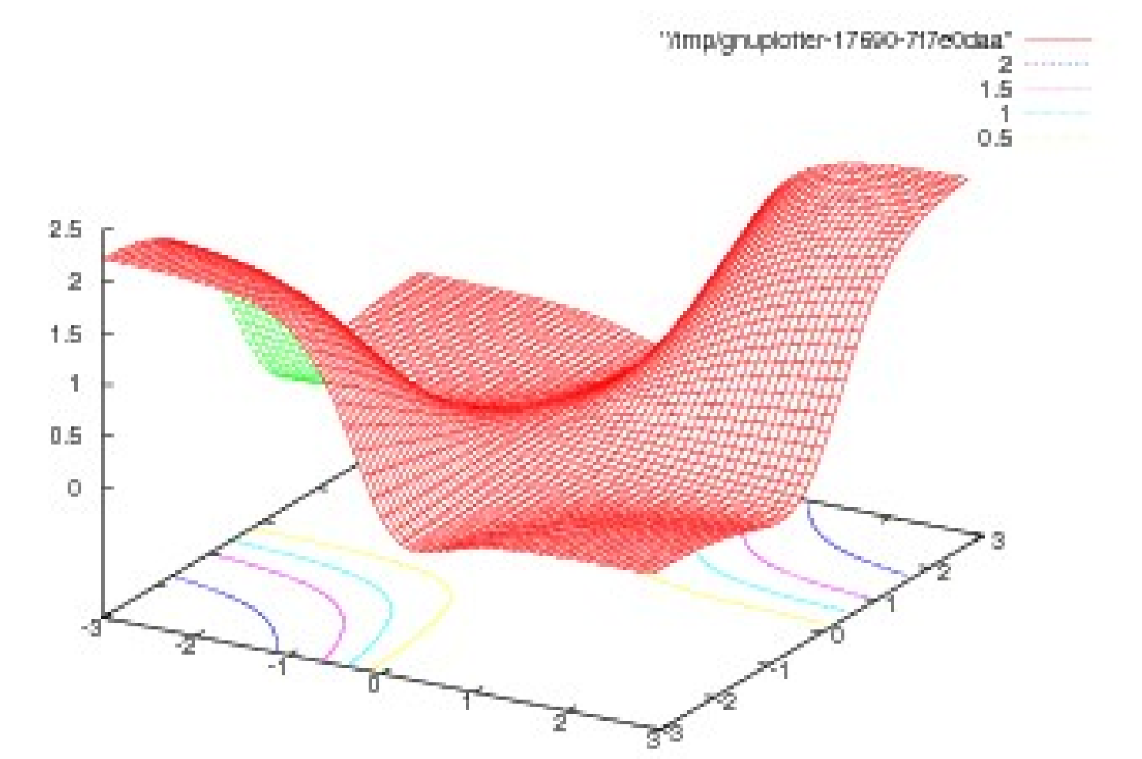
\includegraphics[width=100mm]{lectures/02-b/Identity.PNG}
\caption{Gradient Descent vs. Stochastic Gradient Descent}
\label{fig:sgd}
\end{figure}

Neural networks with at least one non-linear activation function in its hidden layer(s) will have non-convex loss surfaces. 
Convex optimization methods do not work if there are more than one global minimum. 
In this instance, we get two solutions symmetrical to both sides of the saddle point. 
Those solutions are essentially hyperbolas, because if we didn't have the hyperbolic tangents and it was completely linear then we can add one value for the weight $W_0$ and the inverse value for weight $W_1$ and get the identity function. 
For instance if we set $W_0$ to 2 and $W_1$ to $\frac{1}{2}$ and forget about the hyperbolic tangents then we get an identity function.\\

We can choose both positive and negative weights and still get a solution as we have the other solution space on the other side. 
This network has a very highly non-convex objective function where if we start at point that are small distance apart from each other, we can end into different local minima. 
Actually those two minima are equivalent so it does not matter where we start. 
There is empirical evidence that in neural networks it is very often the case, that there are lots of different solutions but they are basically equivalent. \\

Even if we have a simpler version without hyperbolic tangent and completely linear functions, still we see that the solution is similar. 
One other explanation for why regularizers are bad in the beginning of the training is that when we initialize the weights, we have to make sure the weights are initialized to non-zero values since otherwise the learning never takes off and it stays at a saddle point where there is no gradient.
Similarly the backpropagation with zero weights do not update anything and the neural net never takes off. 
The magnitude of the weights is very important and we must pay special attention that we initialize them appropriately.\\

The intuition behind this is that if you have a unit with many inputs that are normalized then the weighted sum of this unit is the weighted sum of random variables with standard deviation/variance one.
The variance of the output will thus be the weighted sum of the variance of the inputs. 
The variance of the weighted sum will be the sum of the variances of the inputs multiplied by the square of the weights. 
If we want our output to have variance once to preserve the variance, then we need to set the weights accordingly - to smaller values if we have many inputs and to bigger values if we have fewer inputs.
Scaling the weights with a factor that is $\frac{1}{\sqrt{N}}$ would preserve variance of inputs in different layers. 
